\chapter{Trainieren des ersten Neuronale Netzes}
In dem vorherigen Kapitel haben wir gesehen,
was Maschinelles Lernen bedeutet, welche
Probleme es hilft zu lösen und warum sich
Deep Learning in der heutigen Zeit mehr und mehr durchsetzt.
Es konnte außerdem das Ziel dieser Arbeit
beschrieben und einen ersten Einblick
in die verwendete Hardware gegeben werden.
In diesem Kapitel soll es darum gehen, die
TensorFlow Bibliothek kennenzulernen
und zu zeigen wie ein Deep-Learning-Modell
für mobile Geräte (und der Google Coral Edge TPU) bereitgestellt wird.
Das Kapitel ist gegliedert nach den folgenden Schritten:
\begin{enumerate}
  \item Hole den Trainingsdatensatz.
  \item Trainiere ein neuronales Netz mit TensorFlow.
  \item Bewerte die Ergebnisse des Modells.
  \item Verbessere das Modell.
  \item Konvertiere das Modell in ein mobil- und TPU-kompatibles Format.
  \item Schreibe ein Programm, um auf dem Gerät Prognosen durchzuführen.
  \item Vergleiche die Ergebnisse und Inferenzgeschwindigkeiten.
\end{enumerate}
Die Idee dieses Kapitels stammt aus Kapitel 4 des Buchs \citetitle{book:tiny-ml}
von \textcite{book:tiny-ml} (welche involviert in der Entwicklung
der TensorFlow Lite Bibliothek sind) mit einigen
anwendungs- und hardwarespezifischen Änderungen.

\section{Das Ziel des Modells}
Ähnlich wie \autoref{sec:lernmethoden} handelt es sich
um ein einfaches Modell mit nur einer Ein- und Ausgabe.
Die zu modellierenden Daten sind etwas komplexer,
es geht um eine bekannte trigonometrische Funktion: der Sinuskurve.
Das Ziel des Modells ist es also, durch eine Eingabe $x$
den $y$ Wert $\sin(x)$ zu bestimmen.
In einer echten Anwendung könnte
diese Zahl natürlich direkt ermittelt werden,
das Beispiel soll jedoch zeigen,
wie mit Deep Learning (und sehr kleinen Netzen)
bereits anspruchsvollere, nicht lineare Daten gut modelliert werden können.
Die Sinusfunktion hat den folgenden Verlauf:
\begin{figure}[h!]
  \centering
  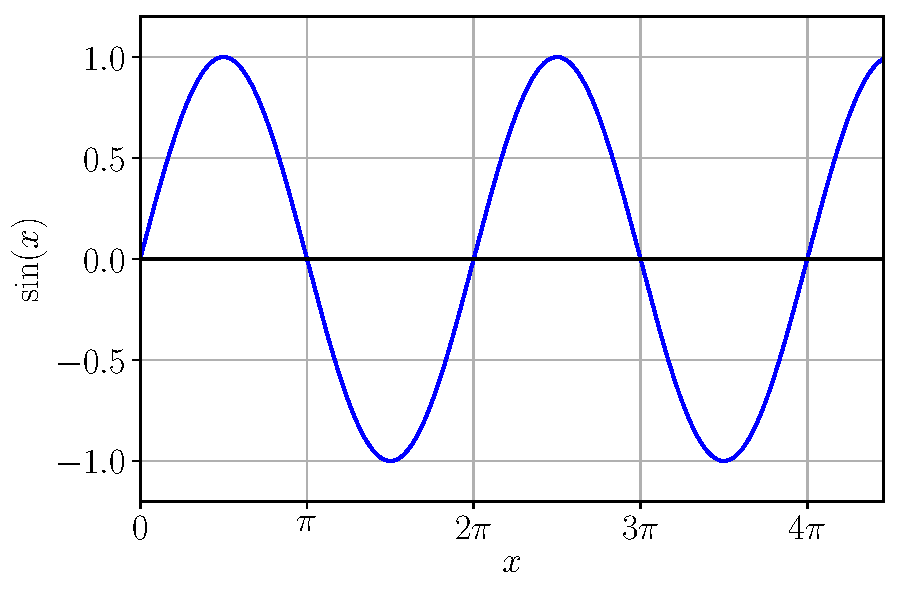
\includegraphics[width=\wMD]{first-nn/sine-curve.pdf}
  \caption{Die Sinusfunktion}
  \label{plot:sine-curve}
\end{figure}

\section{Generieren der Daten}
Neuronale Netze können komplexe Muster in den zugrundeliegenden Daten erkennen
und dabei sehr vielseitig eingesetzt werden.
In diesem Beispiel geht es wie zuvor um ein einfaches Regressionsproblem,
ein neuronales Netz kann genauso gut, aber auch für
Klassifizierung, Bildanalyse, Videoanalyse, unüberwachtes Lernen und vieles mehr verwendet werden.
Die Trainingsdaten werden mit TensorFlow generiert und
die Vorgehensweise ist hierbei sehr ähnlich
wie mit der Verwendung von NumPy:
\begin{pythoncode}
import tensorflow as tf
import math

SAMPLES = 2000

tf.random.set_seed(42)

x = tf.random.uniform((SAMPLES, 1), minval=0, maxval=2*math.pi)
tf.random.shuffle(x)

y = tf.math.sin(x)
\end{pythoncode}
Der vorhergehende Programmausschnitt generiert zwei Spaltenvektoren
(Trainingsdaten \pythoninline{x} und Label \pythoninline{y})
mit jeweils 2000 Werten im Bereich 0 bis $2\pi$.
Dieser Bereich nennt sich die Periode der Sinusfunktion,
da sich die Funktionswerte von dort an immer wiederholen.
Damit das Problem realistischer ist, wird auch für diese Daten
zufälliges Rauschen hinzugefügt:
\begin{pythoncode}
y += 0.25 * tf.random.normal(y.shape)
\end{pythoncode}
\begin{figure}[h!]
  \centering
  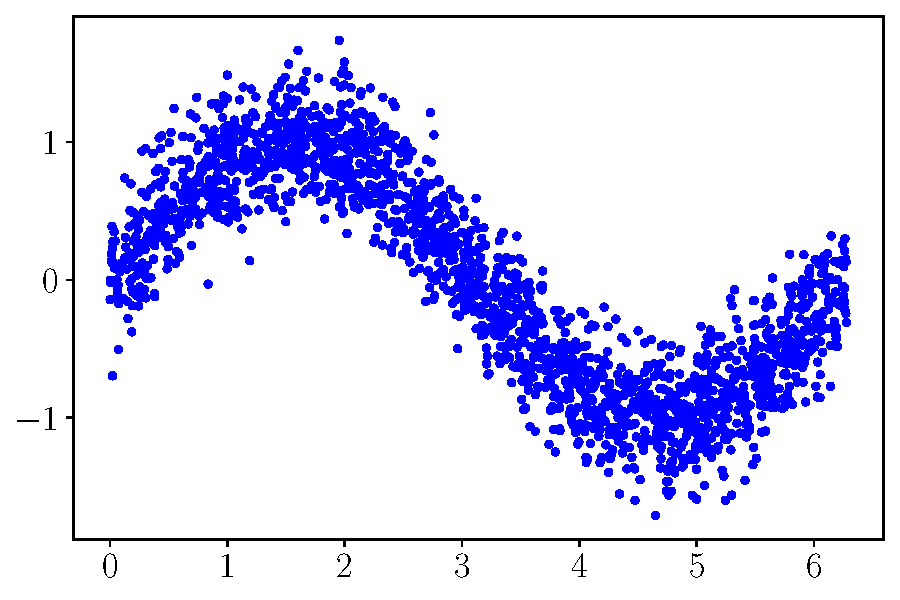
\includegraphics[width=\wMD]{first-nn/sine-data-noise.pdf}
  \caption{Die generierten Sinusdaten plus zufälliges Rauschen}
\end{figure}

\section{Aufteilen der Trainingsdaten}
\label{sec:split-train-data}
Um die Qualität eines Modells bewerten zu können, werden
mehr Daten benötigt als lediglich die Trainingsbeispiele.
Dies ist der Grund warum es für gewöhnlich mehr als nur einen
Datensatz gibt. Eine typische Vorgehensweise ist die Aufgliederung
in drei Teile: dem \textit{training}, \textit{validation} und \textit{test set}.
Die Schritte, um ein passendes Netz für ein Problem zu finden, sind die Folgenden:
\begin{enumerate}
  \item Probiere verschiedene Ideen aus und trainiere einige Modelle mithilfe des
        \textit{training set}.
  \item Bewerte die Qualität der Modelle anhand des \textit{validation set} und wähle
        einen oder mehrere der vielversprechendsten Kandidaten aus.
  \item Verbessere die Leistung der ausgewählten Modelle am \textit{validation set}
        solange, bis ein Modell mit der gewünschten Qualität gefunden wurde.
        Das ausgewählte Modell kann schließlich durch das
        \textit{test set} evaluiert werden, um den Generalisierungsfehler abzuschätzen.
\end{enumerate}
Im Training sollte der Algorithmus lediglich die Trainingsdaten
zu Gesicht bekommen. Dies hilft bekannten
Fehlerquellen wie der Überanpassung (dem Gegenstück zur Unteranpassung, engl.
\textit{overfitting} und \textit{underfitting}) vorzubeugen.
Die folgende Abbildung soll die beiden Begriffe deutlich machen:
\begin{figure}[h!]
  \centering
  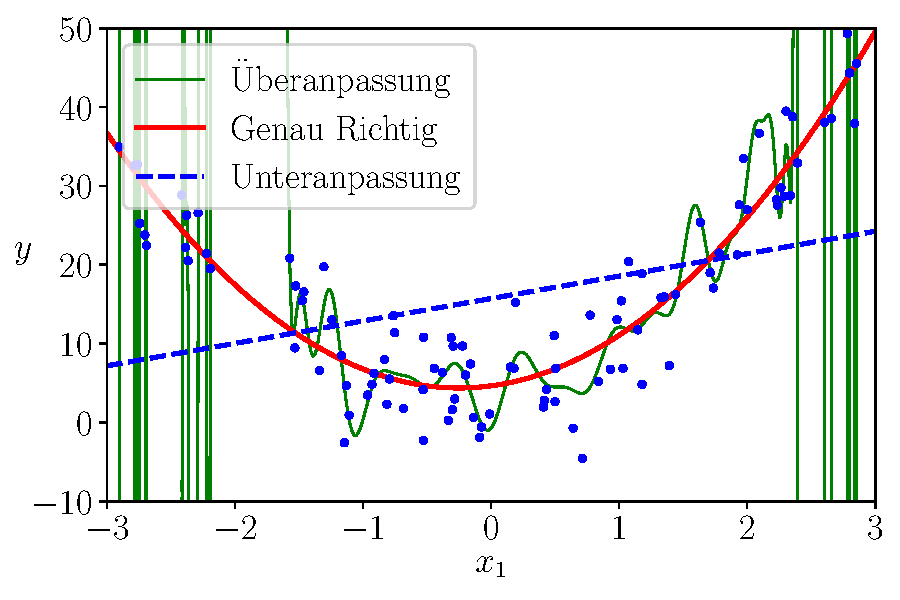
\includegraphics[width=\wLG]{first-nn/over_underfitting.pdf}
  \caption{Überanpassung und Unteranpassung am Beispiel einer
  quadratischen Funktion \parencite[131]{book:hands-on-ml}}
\end{figure}

\noindent
Modelliert ein Algorithmus die Struktur der Trainingsdaten zu gut, dann
ist die Rede von Überanpassung. Dies ist zu sehen
durch die grüne Linie. Die Funktion mit sehr vielen Features
mag die Trainingsdaten am besten beschreiben,
schafft es aber nicht auf neue Punkte zu verallgemeinern.
Überanpassung kann erkannt werden, wenn die Leistung des Modells am
\textit{training set} steigt, während sie am \textit{validation set}
sinkt. Das Gegenstück der Überanpassung ist die
Unteranpassung. Dies ist zu sehen durch die blau gestreifte Linie.
Das Modell (mit nur linearen Features)
schafft es nicht die Datenverteilung gut genug zu beschreiben.
Die besten Ergebnisse werden in diesem Beispiel durch die rote Linie erzeugt.
Um die zuvor generierten Trainingsdaten aufzuteilen,
kann die TensorFlow Methode \pythoninline{tf.split}
verwendet werden:
\begin{pythoncode}
# Wir verwenden 50% der Daten für training und 30% für testing.
# Die restlichen 20% werden für validation verwendet.
TRAIN_SIZE = int(0.5 * SAMPLES)
TEST_SIZE = int(0.3 * SAMPLES)
VAL_SIZE = SAMPLES - TRAIN_SIZE - TEST_SIZE

# Gliedere den Datensatz in drei Teile auf
x_train, x_test, x_val = tf.split(x, [TRAIN_SIZE, TEST_SIZE, VAL_SIZE])
y_train, y_test, y_val = tf.split(y, [TRAIN_SIZE, TEST_SIZE, VAL_SIZE])

# Verifiziere die Aufteilung, durch summieren der Größen
assert tf.size(x_train) + tf.size(x_test) + tf.size(x_val) == SAMPLES
\end{pythoncode}
Die resultierenden Datensätze können farblich dargestellt werden:
\begin{figure}[h!]
  \centering
  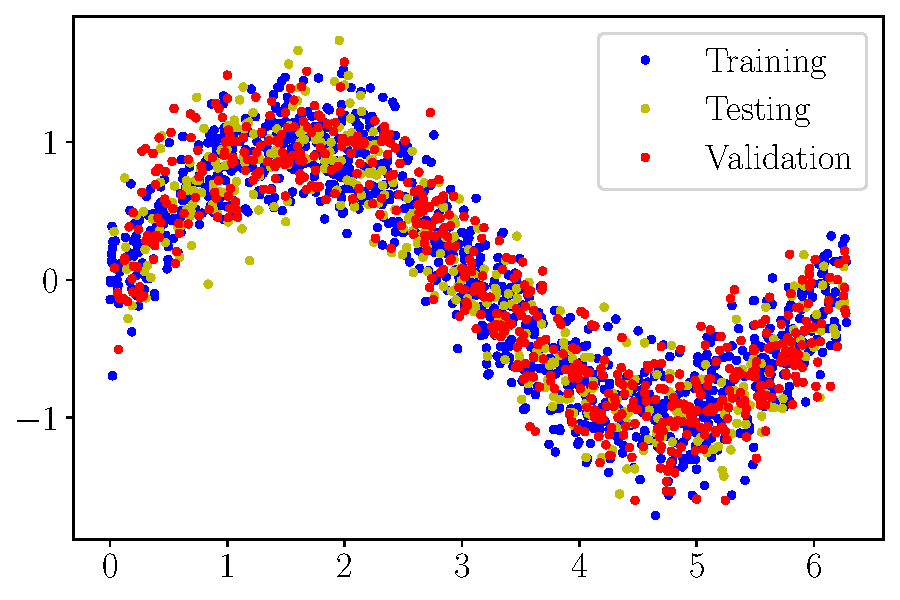
\includegraphics[width=\wMD]{first-nn/sine-data-noise-split.pdf}
  \caption{Aufteilung der Sinusdaten in
  \textit{training}, \textit{validation} und \textit{test set}}
\end{figure}

\section{Entwurf des ersten Modells}
\label{sec:modellentwurf}
Ein neuronales Netz besteht aus mehreren kleinen Einheiten (auch Neuronen genannt).
Jedes Neuron nimmt entgegen ein bis $n$ numerische Eingaben, führt einige
einfache Berechnungen durch und produziert eine numerische Ausgabe.
Alleine kann ein Neuron kaum die einfachsten Probleme lösen, doch zusammen
durch Komposition und Training haben sie das Potenzial,
die komplexe Welt zu verstehen.
Der Aufbau eines einzelnen Neuron ist in \autoref{fig:nn-neuron} zu sehen.
\begin{figure}[h!]
  \centering
  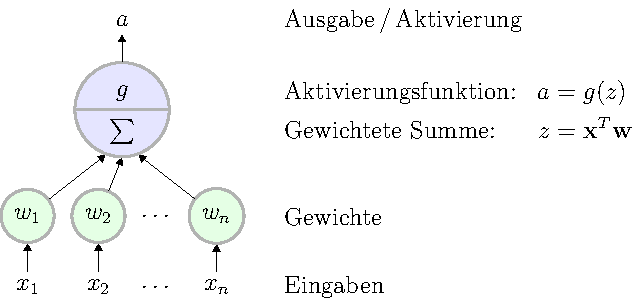
\includegraphics{first-nn/nn-neuron.pdf}
  \caption{Der Aufbau eines einzelnen Neuron}
  \label{fig:nn-neuron}
\end{figure}

\noindent
Als erster Schritt wird eine gewichtete Summe
($z = w_1x_1 + w_2x_2 +\dotsb+ w_nx_n + b = \mathbf{x}^T\mathbf{w} + b$)
der Eingabewerte plus Bias-Wert berechnet. Die Elemente $\mathbf{x}$ und $\mathbf{w}$
sind Spaltenvektoren der Form: $(x_1,\dotsc,x_n)^T$ und $(w_1,\dotsc,w_n)^T$.
\footnote{Wie immer wird versucht Berechnungen als Vektor- und Matrixoperationen
auszudrücken um CPU und GPU Beschleunigung auszunutzen.}
Der zweite Schritt wendet eine Aktivierungsfunktion auf diese Summe an und dies
erzeugt die Ausgabe: $a = g(z)$. Die Ausgabe eines Neurons
wird typischerweise die Aktivierung genannt. Ein neuronales Netz
besteht aus der Komposition verschiedener Neuronen und die
Gewichte und Bias-Werte stellen die erlernbaren Parameter dar.
\begin{figure}[h!]
  \centering
  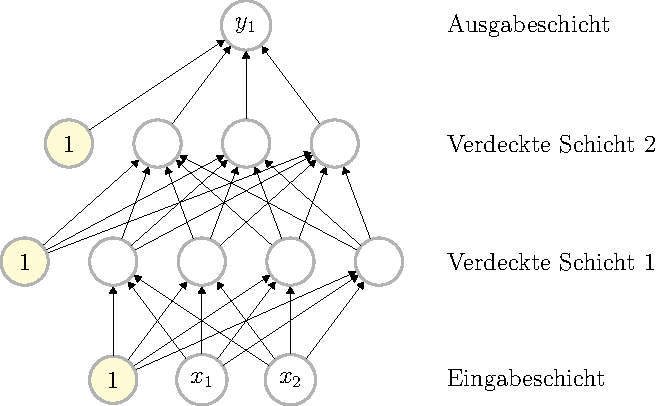
\includegraphics{first-nn/example-nn.pdf}
  \caption{Ein einfaches neuronales Netz mit zwei verdeckten Schichten}
  \label{fig:example-nn}
\end{figure}
\noindent
\autoref{fig:example-nn} zeigt ein einfaches neuronales Netz
mit zwei verdeckten Schichten (engl. \textit{hidden layers}),
zwei Eingaben und einer Ausgabe.
Verdeckte Schichten sind all diejenigen Schichten, die nicht Ein- oder Ausgabe sind.
Jede Schicht außer der Ausgabeschicht enthält ein Bias-Neuron
(in Gelb markiert), welches immer Eins ausgibt, aber auch trainiert werden kann
und ist vollständig mit der nächsten Schicht verbunden.
Ein neuronales Netz wird tief genannt, wenn es viele verdeckte Schichten besitzt.
\footnote{In den 1990er-Jahren wurde ein neuronales Netz
mit mehr als zwei verdeckten Schichten als tief angesehen.
Da es aber heutzutage Netze mit Dutzend und Hunderten von Schichten
gibt, ist die Definition von \enquote{tief} etwas schwammig \parencite[289]{book:hands-on-ml}.}
Es wird durch einen Algorithmus trainiert, der
sich Backpropagation nennt.
Backpropagation ist der weitaus mathematischste Teil von
Deep Learning, da der Schwerpunkt dieser Arbeit auf der Entwicklung einer
Anwendung liegt, werden wir nicht im Detail untersuchen,
wie dieser und verwandte Algorithmen wie das Gradientenabstiegsverfahren
funktionieren. Zusätzlich können diese Methoden durch Deep-Learning-Bibliotheken
wie TensorFlow automatisiert werden. Es wird jedoch versucht, einige
Intuitionen zu geben.\\[8pt]
Kurzum \parencite[290-291]{book:hands-on-ml}:
Backpropagation besteht aus zwei Phasen: einem Vorwärtsdurchlauf
und einem Rückwärtsdurchlauf. Die Daten werden stapelweise verarbeitet
(\zB{} 32 Datensätze auf ein­mal) und der gesamte Trainingsdatensatz
wird mehrfach durchlaufen. Ein Trainingsdurchlauf nennt sich Epoche.\\[4pt]
Jeder Datenstapel wird an die erste Schicht des neuronalen Netzes
übergeben. Von dort wird im Vorwärtsdurchlauf die Aktivierung aller
Neuronen bis hin zur Ausgabeschicht ermittelt und die Zwischenerbnisse gespeichert.\\[4pt]
Nachdem die Ausgaben der letzten Schicht bekannt sind, kann
durch Vergleich der Sollwerte der Fehler des Netzes ermittelt werden.
Dies geschieht durch eine Kostenfunktion $J$. Im Fall eines Regressionsproblems
wird typischerweise die mittlere quadratische Abweichung verwendet
(engl. \textit{mean squared error}) \parencite[113-114]{book:hands-on-ml}:
\begin{equation}
  J(\mathbf{\hat{y}}, \mathbf{y}) =
  MSE(\mathbf{\hat{y}}, \mathbf{y}) =
    \frac{1}{m} \sum_{i=1}^{m} (\mathbf{\hat{y}}^{(i)} - \mathbf{y}^{(i)})^2
  \label{eq:mse}
\end{equation}
Die Elemente $\mathbf{\hat{y}}$ und $\mathbf{y}$ sind Spaltenvektoren
mit den Ausgaben des Netzes und den tatsächlichen Werten, die Zahl $m$
ist die Größe des Vektors, welche in diesem Fall gleich der Stapelgröße
(engl. \textit{batch size}) ist. Der Index $\mathbf{v}^{(i)}$ ist keine Potenz,
sondern beschreibt den i-ten Wert im Vektor $\mathbf{v}$.\\[4pt]
Der Rückwärtsdurchlauf im letzten Schritt ist der eigentliche Teil,
mit dem das Netz
trainiert wird. Der Algorithmus misst, wie stark jedes Gewicht den Fehler der
vorherigen Schicht beeinflusst hat und versucht, diese so anzupassen,
damit die Kostenfunktion minimiert wird.\\[8pt]
TensorFlow und insbesondere die TensorFlow Keras API
machen es einfach, neuronale Netze zu entwerfen und zu trainieren.
Keras ist eine High-Level Deep Learning API, welche
von François Chollet als Teil eines Forschungsprojekts entwickelt
wurde und seit März 2015 ein Open-Source-Projekt ist
\parencite[295]{book:hands-on-ml}. Keras kann
unabhängig von TensorFlow verwendet werden, es benötigt
jedoch eine Berechnungsgrundlage (wie TensorFlow und Co.),
mit der die für DL erforderlichen
rechenintensiven Operationen durchgeführt werden können.
In dieser Arbeit wird daher ausschließlich die \pythoninline{tf.keras} API
verwendet. Ein Modell mit Keras zu entwerfen ist unkompliziert:
\begin{pythoncode}
from tensorflow import keras

input_layer = keras.layers.Input(shape=[1])
hidden1 = keras.layers.Dense(units=16, activation="relu")(input_layer)
output_layer = keras.layers.Dense(units=1, name="output")(hidden1)

model = keras.Model(inputs=input_layer, outputs=output_layer)
\end{pythoncode}
\begin{itemize}
  \item Die erste Zeile importiert das Keras Modul von TensorFlow.
  \item Als nächstes wird die Eingabeschicht des Netzes definiert.
        Diese dient ausschließlich dazu, die Dimension der Eingabewerte festzulegen.
        Da das Modell nur eine einzige Zahl entgegen nimmt,
        ist die Dimension des Eingabevektors eins.
  \item Die nächste Zeile definiert die erste und einzige verborgene Schicht mit
        16 Neuronen (\textit{units}). Die Neuronen verwenden die ReLU
        (\textit{Rectified Linear Unit}) Aktivierungsfunktion, welche wie folgt
        definiert ist:
        \begin{equation}
          g(z) = ReLU(z) = \max(0, z)
        \end{equation}
        ReLU ist eine sehr beliebte Aktivierungsfunktion, die sich nicht
        nur einfach berechnen lässt, sondern auch in der Praxis bewährt hat
        und daher gut als Standardauswahl eignet. Es gibt viele
        weitere Aktivierungsfunktion, welche häufig eingesetzt werden.
        Vier der Gewöhnlichsten sind in \autoref{fig:activation-functions}
        zu sehen, wobei die Heaviside-Schwellenwertfunktion aufgrund der
        historischen Relevanz aufgenommen wurde.
        \begin{figure}[h!]
          \centering
          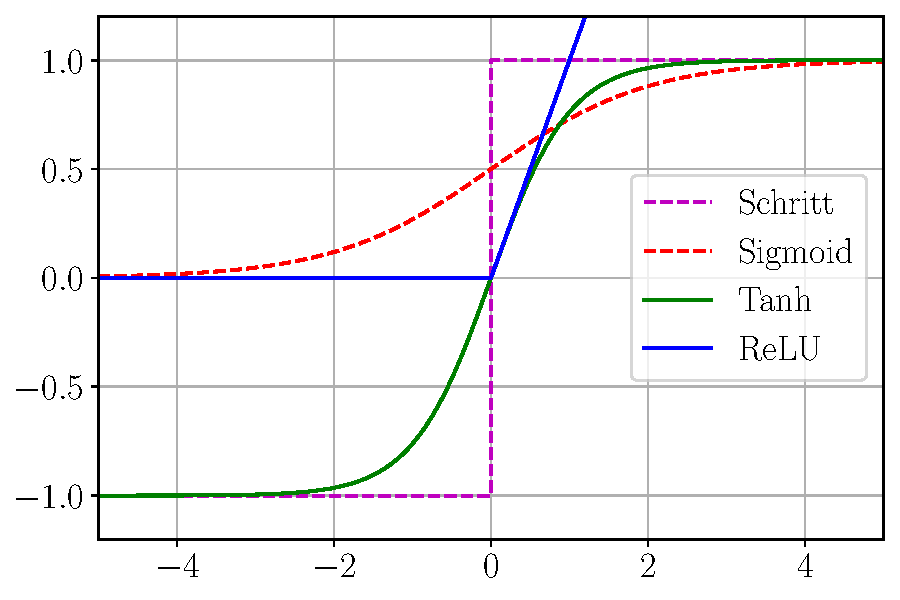
\includegraphics[width=\wMD]{first-nn/activation-functions.pdf}
          \caption{Verschiedene Aktivierungsfunktionen \parencite[292]{book:hands-on-ml}}
          \label{fig:activation-functions}
        \end{figure}
  \item Die letzten beiden Zeilen definieren die Ausgabeschicht und das endgültige
        Modell. Da das Ziel ist, einen einzigen Wert zu bestimmen, besitzt die letzte
        Ebene lediglich eine Einheit. Es wird keine Aktivierungsfunktion angegeben,
        was bedeutet, dass die Identitätsfunktion verwendet wird:
        \begin{equation}
          g(z) = z
        \end{equation}
\end{itemize}
Die \pythoninline{model.summary()} Funktion liefert einige nützliche Informationen
über das erstellte Netz, wie die verschiedenen Schichten, die Dimension
der Aktivierungen (\pyconinline{None} bedeutet eine beliebige Stapelgröße)
und die Anzahl der Parameter:
\begin{pyconcode}
>>> model.summary()
Model: "model"
_________________________________________________________________
Layer (type)                 Output Shape              Param #   
=================================================================
input_1 (InputLayer)         [(None, 1)]               0         
_________________________________________________________________
dense (Dense)                (None, 16)                32        
_________________________________________________________________
output (Dense)               (None, 1)                 17        
=================================================================
Total params: 49
Trainable params: 49
Non-trainable params: 0
_________________________________________________________________
\end{pyconcode}
Die erste verdeckte Schicht mit einer Eingabe und 16 Ausgaben besitzt
32 Parameter, 16 Gewichte ($\#Eingaben \cdot \#Ausgaben$) und 16 Bias-Werte ($\#Ausgaben$).
Die Ausgabeschicht mit 16 Eingaben und einer Ausgabe, besitzt
17 Parameter, 16 Gewichte und ein Bias-Wert.
Auf die einzelnen Schichten kann per Index oder Name zugegriffen werden:
\begin{pyconcode}
>>> model.layers
[<tensorflow.python.keras.engine.input_layer.InputLayer at 0x225b4ca4310>,
 <tensorflow.python.keras.layers.core.Dense at 0x225b4cb96d0>,
 <tensorflow.python.keras.layers.core.Dense at 0x227629dea30>]
>>> hidden1 = model.layers[1]
>>> hidden1.name
dense
>>> model.get_layer("dense") is hidden1
True
\end{pyconcode}
Die Parameter einer Schicht können ebenfalls untersucht werden,
hierfür gibt es Funktionen wie
\pythoninline{get_weights()} und \pythoninline{set_weights()}:
\begin{pyconcode}
>>> weights, biases = hidden1.get_weights()
>>> weights
array([[ 0.5445634 , -0.5741172 , -0.2190957 , -0.40382388,  0.25530386,
         0.34373027, -0.45763797, -0.1983017 , -0.3434852 ,  0.14649397,
         0.57805157, -0.4487671 , -0.34861064,  0.44097137, -0.5695514 ,
        -0.33477765]], dtype=float32)
>>> weights.shape
(1, 16)
>>> biases
array([0., 0., 0., 0., 0., 0., 0., 0., 0., 0., 0., 0., 0., 0., 0., 0.],
      dtype=float32)
>>> biases.shape
(16,)
\end{pyconcode}
Es ist zu sehen, dass die Gewichte der Ebene zufällig initialisiert wurden.
Dies ist wichtig, um die Symmetrie der Verbindungen zu brechen,
da sonst der Backpropagation-Algorithmus alle Gewichte gleichbehandeln würde
und das Training ineffektiv ist \parencite[291]{book:hands-on-ml}.
Für die Bias-Werte ist es in Ordnung, mit null zu initialisieren.
Nachdem das Modell erstellt wurde, kann die \pythoninline{model.compile()}
Methode aufgerufen werden, um die Kostenfunktion und den
Optimierungsalgorithmus festzulegen.
Als alternatives drittes Argument kann eine Liste von
zusätzlichen Messwerten angegeben werden:
\begin{pythoncode}
sgd = keras.optimizers.SGD()
model.compile(optimizer=sgd, loss="mse", metrics=["mae"])
\end{pythoncode}
Als Kostenfunktion wird die mittlere quadratische Abweichung verwendet
\eqref{eq:mse} und der Optimierungsalgorithmus ist
\textit{stochastic gradient descent} (SGD). \textit{Gradient descent}
(dt. Gradientenabstieg) ist ein allgemeiner Optimierungsalgorithmus
um eine Kostenfunktion zu minimieren \parencite[118]{book:hands-on-ml}.
Es soll in dieser Arbeit nicht im Detail untersucht werden, wie dieser
Algorithmus funktioniert, nichtsdestotrotz sind einige Intuitionen
in \autoref{appx:gradient-descent} gegeben.
Als zusätzlicher Messwert wird die mittlere absolute Abweichung
(engl. \textit{mean absolute error}) angegeben.
Die Gleichung ist sehr ähnlich wie die des $MSE$ nur das der absolute Fehler
anstelle des quadratischen Fehlers gemessen wird:
\begin{equation}
  J(\mathbf{\hat{y}}, \mathbf{y}) =
  MAE(\mathbf{\hat{y}}, \mathbf{y}) =
    \frac{1}{m} \sum_{i=1}^{m} \vert\mathbf{\hat{y}}^{(i)} - \mathbf{y}^{(i)}\vert
  \label{eq:mae}
\end{equation}
Die mittlere absolute Abweichung ist vor allem für ein Regressionsproblem
ein gutes Maß, um abzuschätzen, wie stark Prognosen im Training von
den Sollwerten abweichen.

\section{Das Modell trainieren und bewerten}
\label{sec:train-evaluate-model}
Das Netz ist nun bereit um trainiert zu werden.
Dies funktioniert durch den Aufruf der \pythoninline{fit} Methode:
\begin{pyconcode}
>>> EPOCHS = 300
>>> BATCH_SIZE = 16
>>> history = model.fit(x_train, y_train, epochs=EPOCHS,
...                     batch_size=BATCH_SIZE, validation_data=(x_val, y_val))
...
Epoch 1/300
63/63 [======] - 2s 4ms/step - loss: 0.5319     - mae: 0.6028
                             - val_loss: 0.3661 - val_mae: 0.5134
Epoch 2/300
63/63 [======] - 0s 3ms/step - loss: 0.3422     - mae: 0.4941
                             - val_loss: 0.2898 - val_mae: 0.4533
[...]
Epoch 300/300
63/63 [======] - 0s 3ms/step - loss: 0.2138     - mae: 0.3667
                             - val_loss: 0.2135 - val_mae: 0.3671
\end{pyconcode}
Es wird das \textit{training set} angegeben und die Epochenzahl
und Stapelgröße festgelegt.
Als optionales Argument wird außerdem das \textit{validation set}
übergeben. Die Stapelgröße zeigt, wie viele Trainingsdaten betrachten werden,
bevor die Kostenfunktion bestimmt und die Gewichte und Bias-Werte
des Netzes einmal angepasst werden
(wie häufig ein Schritt des Gradientenabstiegs durchgeführt wird).
In \autoref{sec:split-train-data} wurden \qty{50}{\percent} der Daten
als \textit{training set} verwendet:
\begin{pyconcode}
>>> x_train.shape # 2000 * 50% = 1000
TensorShape([1000, 1])
\end{pyconcode}
Wie in der oberen Ausgabe zu sehen ist, macht dies
pro Epoche 63 ($1000 / 16 = \num{62.5}$) Gewichts- und Bias-Aktualisierungen.
Durch erneutes Betrachten der Parameter nach dem Training
können die Veränderungen beobachtet werden:
\begin{pyconcode}
>>> hidden1 = model.get_layer("dense")
>>> weights, biases = hidden1.get_weights()
>>> weights
array([[ 0.48667157, -0.5741172 , -0.2190957 , -0.40382388,  0.43343386,
         0.23612383, -0.45763797, -0.1983017 , -0.3434852 ,  0.7860139 ,
         0.55660063, -0.4487671 , -0.34861064,  0.41839647, -0.5695514 ,
        -0.33477765]], dtype=float32)
>>> biases
array([-0.6504982 ,  0.        ,  0.        ,  0.        , -0.5743109 ,
       -0.00350828,  0.        ,  0.        ,  0.        , -0.9752765 ,
       -0.00748946,  0.        ,  0.        , -0.00579908,  0.        ,
        0.        ], dtype=float32)
\end{pyconcode}
Nicht alle Parameter der verdeckten Schicht wurden angepasst, einige
Änderungen an den Bias-Werten sind jedoch gut zu erkennen.
Die Keras Ausgabe enthält weitere nützliche Informationen:
\begin{description}[font=\normalfont, style=nextline]
\item[\pyconinline{loss} und \pyconinline{val_loss}]
Die Ausgabe der Kostenfunktion für das \textit{training} und \textit{validation set}.
Es ist zu erkennen, dass der Fehler während
dem Training für beide Datensätze abnimmt,
was ein gutes Zeichen ist.
\item[\pyconinline{mae} und \pyconinline{val_mae}]
Die mittlere absolute Abweichung. Wie auch die Kostenfunktion
nimmt diese für beide Datensätze während dem Training ab.
Ein absoluter Fehler von \num{0.3667}
nach 300 Epochen ist allerdings noch immer relativ hoch.
Angesichts der Tatsache, dass mögliche Werte ungefähr im
Bereich $[-1, 1]$ liegen.
Dies könnte bedeuten, dass es das Netz nicht geschafft hat, die Daten
gut zu modellieren. Mehr Einblicke können erlangt werden, sobald
das Modell getestet und die Ergebnisse grafisch dargestellt werden.
\end{description}

\subsection{Grafische Darstellung des Trainings}
Die \pythoninline{fit} Methode gibt ein \pythoninline{History} Objekt zurück.
Ihr \pythoninline{History.history} Attribut
ist eine Aufzeichnung aller Messwerte in aufeinanderfolgenden Epochen:
\begin{pyconcode}
>>> history.history.keys()
dict_keys(["loss", "mae", "val_loss", "val_mae"])
>>> mse = history.history["loss"]
>>> val_mse = history.history["val_loss"]
>>> mae = history.history["mae"]
>>> val_mae = history.history["val_mae"]
>>> len(mse) == len(val_mse) == len(mae) == len(val_mae) == EPOCHS
True
\end{pyconcode}
Diese Aufzeichnungen können verwendet werden um die Trainingswerte
in Bezug auf die Epochenzahl darzustellen:
\begin{pythoncode}
import matplotlib.pyplot as plt

epochs = tf.range(0.0, EPOCHS)

fig, (ax1, ax2) = plt.subplots(2, 1, figsize=[6.4, 8])

# Stelle den MSE für beide Datensätze dar
ax1.plot(epochs, mse, "b-", label="Training")
ax1.plot(epochs, val_mse, "g-", label="Validation")

# Stelle den MAE für beide Datensätze dar
ax2.plot(epochs, mae, "b-", label="Training")
ax2.plot(epochs, val_mae, "g-", label="Validation")

[...] # Achsenbeschriftung, Gitter und Legende

plt.show()
\end{pythoncode}
\begin{figure}[h!]
  \centering
  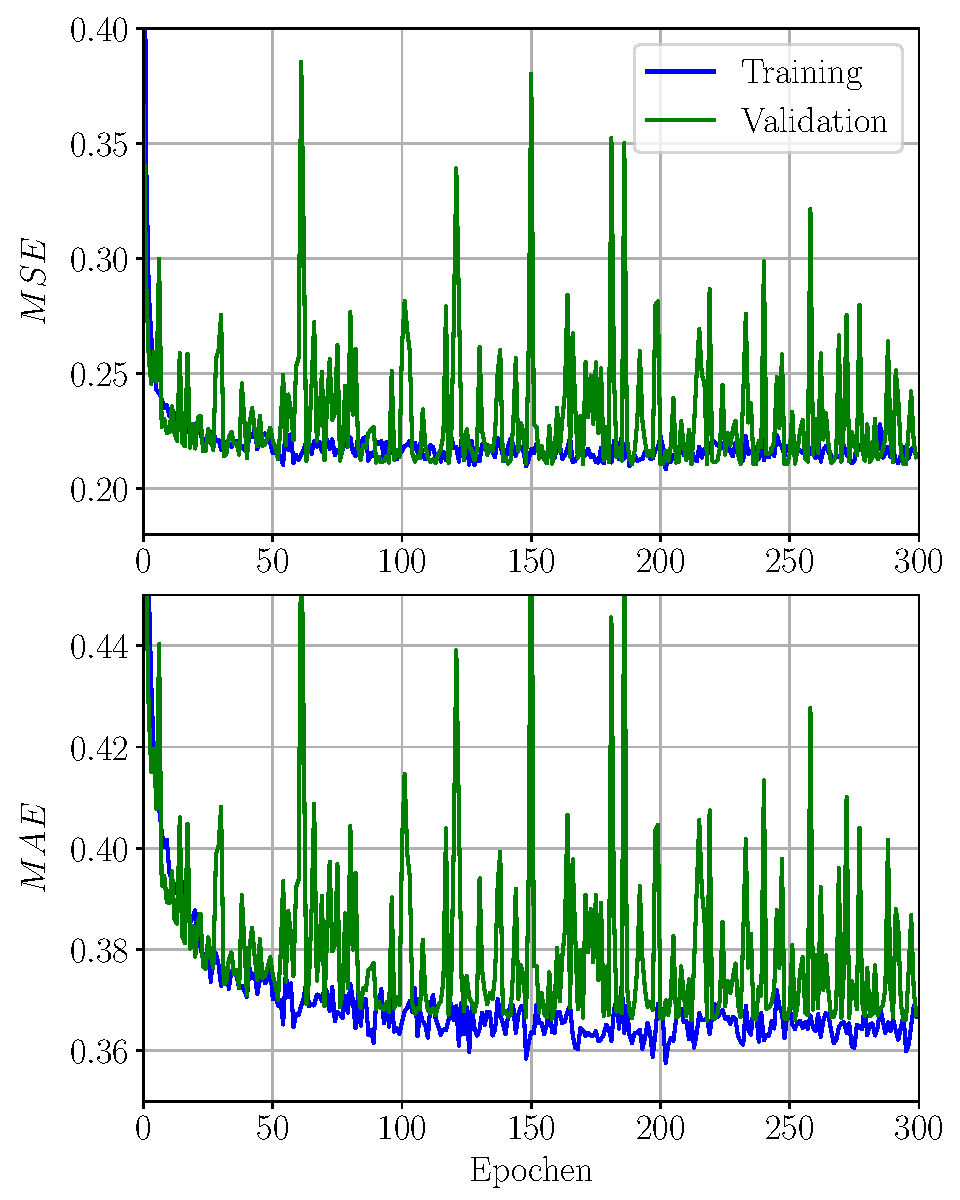
\includegraphics[width=\wMD]{first-nn/1-metrics.pdf}
  \caption{Trainingskurven: Der durchschnittliche \textit{training}
  $MSE$ und $MAE$ gemessen während jeder Epoche
  und der \textit{validation} $MSE$ und $MAE$
  gemessen am Ende jeder Epoche}
\end{figure}
\noindent
Es ist zu sehen, dass beide Fehler sowohl für das
\textit{training set} als auch das \textit{validation set}
zu Beginn des Trainings stark fallen.
Die Werte sind relativ nahe beieinander, wobei die Validierungsfehler
teilweise stark variieren, aber auf keine Überanpassung hin deuten.
Das Modell scheint nach etwa 150 bis 200 Epochen für beide Graphen
keinen großen Fortschritt mehr zu machen, weshalb
das Training bereits frühzeitig beendet werden könnte.
Der Fehler auf dem \textit{validation set} wird
am Ende jeder Epoche gemessen, während der Trainingsfehler als Durchschnittswert
während der Epoche bestimmt wird \parencite[305]{book:hands-on-ml}.
Dies ist der Grund, warum die Validierungsfehler
vereinzelt kleiner als die Trainingsfehler sind:
Das Modell wurde zum Zeitpunkt der Berechnung ein wenig länger trainiert.

\subsection{Grafische Darstellung der Prognosen}
Um die Qualität des Netzes weiter zu beurteilen, können einige
Prognosen mit dem \textit{training} oder \textit{validation set}
durchgeführt und die Ergebnisse angezeigt werden:
\begin{pythoncode}
predictions = model.predict(x_val)

# Zeige die Prognosen zusammen mit den Sollwerten an
plt.plot(x_val, y_val, "b.", label="Validierungsdaten")
plt.plot(x_val, predictions, "y.", label="Prognose")
[...] # Legende und die Daten der Sinuskurve
plt.show()
\end{pythoncode}
\begin{figure}[h!]
  \centering
  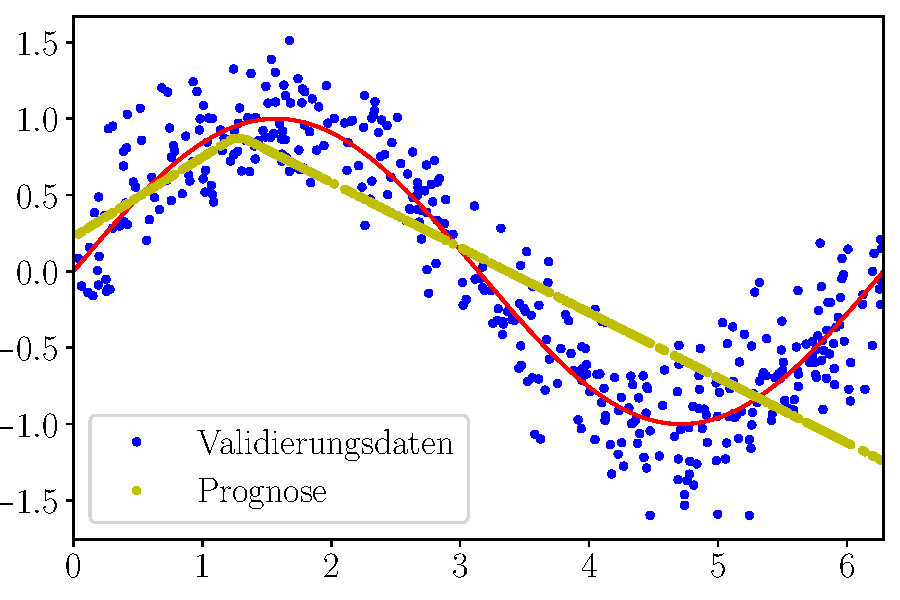
\includegraphics[width=\wMD]{first-nn/1-predictions_val.pdf}
  \caption{Ein Graph der Prognosen des Modells gegenüber der Sollwerte aus dem
  \textit{validation set} zusammen mit der Sinuskurve als Referenz}
  \label{fig:sine-underfitting}
\end{figure}
Oje, \autoref{fig:sine-underfitting} macht die zuvor gestellte Vermutung klar.
Das Modell hat es nur in einer sehr beschränkten Weise
geschafft, die Sinuskurve zu ap­pro­xi­mie­ren.
Es ist also Zeit, zurück ans Zeichenbrett zu gehen und
das Modell anzupassen, um die Qualität am \textit{validation set}
zu verbessern.

\section{Das Modell verbessern}
Es scheint, als wäre das zuvor entworfene Modell nicht mächtig genug,
um die Daten ausreichend gut zu beschreiben.
Um dieser Unteranpassung vorzubeugen, muss die Komplexität des Netzes
erhöht werden. Hierfür gibt es zwei Möglichkeiten:
Hinzufügen weiterer Schichten oder Erhöhen der Neuronenanzahl.
Das Netz soll durch zwei zusätzliche Schichten erweitert werden:
\begin{pythoncode}
input_layer = keras.Input(shape=[1])
# Erste neue Schicht mit 8 Einheiten
hidden1 = keras.layers.Dense(units=8, activation="relu")(input_layer)
# Alte Schicht mit 16 Einheiten
hidden2 = keras.layers.Dense(units=16, activation="relu")(hidden1)
# Zweite neue Schicht mit 32 Einheiten
hidden3 = keras.layers.Dense(units=32, activation="relu")(hidden2)
output_layer = keras.layers.Dense(1, name="output")(hidden3)

model = keras.Model(inputs=input_layer, outputs=output_layer)
\end{pythoncode}
Die Übersicht gibt Auskunft über die Anzahl der Parameter:
\begin{pyconcode}
>>> model.summary()
Model: "model"
_________________________________________________________________
Layer (type)                 Output Shape              Param #   
=================================================================
input_1 (InputLayer)         [(None, 1)]               0         
_________________________________________________________________
dense (Dense)                (None, 8)                 16        
_________________________________________________________________
dense_1 (Dense)              (None, 16)                144       
_________________________________________________________________
dense_2 (Dense)              (None, 32)                544       
_________________________________________________________________
output (Dense)               (None, 1)                 33        
=================================================================
Total params: 737
Trainable params: 737
Non-trainable params: 0
_________________________________________________________________
\end{pyconcode}
737 im Vergleich zu den 49 Parametern des alten Modells.
Dies sollte dem Netz sehr viel mehr Spielraum gegeben,
die Daten gut zu beschreiben.
Das Training funktioniert in gleicherweise wie zuvor:
\begin{pyconcode}
>>> sgd = keras.optimizers.SGD()
>>> model.compile(optimizer=sgd, loss="mse", metrics=["mae"])
>>> history = model.fit(x_train, y_train, epochs=EPOCHS,
...                     batch_size=BATCH_SIZE, validation_data=(x_val, y_val))
...
Epoch 1/300
63/63 [======] - 0s 4ms/step - loss: 0.4988     - mae: 0.6041
                             - val_loss: 0.3944 - val_mae: 0.5356
[...]
Epoch 300/300
63/63 [======] - 0s 4ms/step - loss: 0.0646     - mae: 0.2027
                             - val_loss: 0.0710 - val_mae: 0.2125
\end{pyconcode}
Auch die Trainingskurven werden nach demselben Prinzip
generiert:
\begin{figure}[h!]
  \centering
  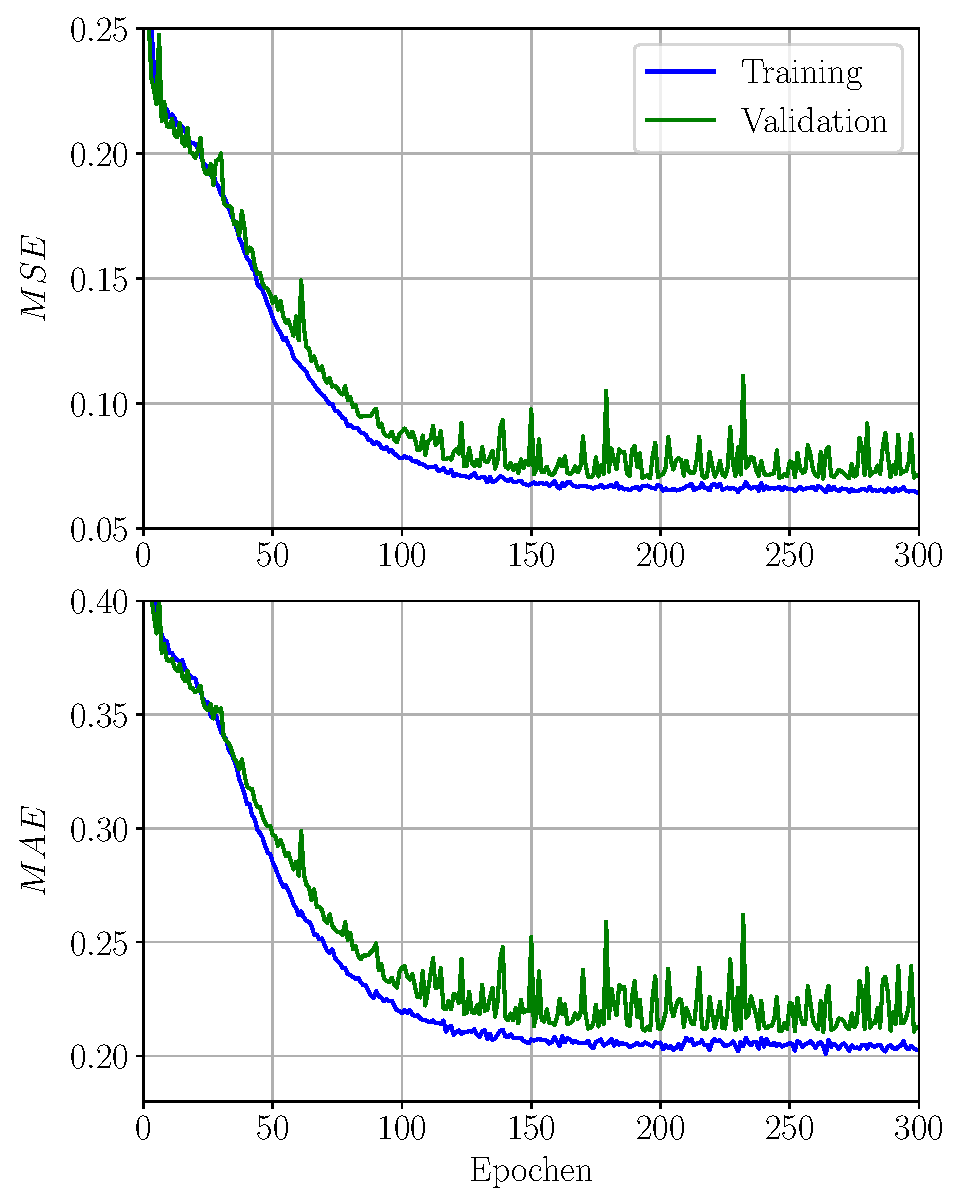
\includegraphics[width=\wMD]{first-nn/2-metrics.pdf}
  \caption{Trainingskurven des angepassten Modells}
\end{figure}

\noindent
Die Trainingsergebnisse sind vielsprechend, sowohl MSE als auch MAE
sind um einiges niedriger als zuvor und die Trainingskurven
sehen allgemein stabiler aus mit weniger großen Ausreißern.
Die grafische Darstellung der Prognosen bestätigt dieses Ergebnis:
\begin{figure}[h!]
  \centering
  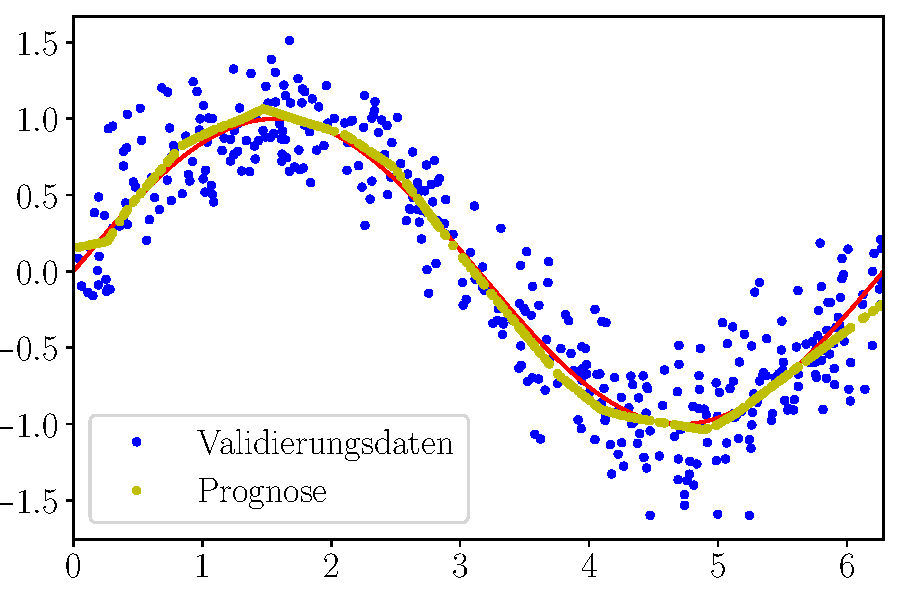
\includegraphics[width=\wMD]{first-nn/2-predictions_val.pdf}
  \caption{Ein Graph der Prognosen des verbesserten Modells gegenüber der Sollwerte aus dem
  \textit{validation set} zusammen mit der Sinuskurve als Referenz}
\end{figure}

\noindent
Das Netz scheint die Daten trotz Rauschen gut beschreiben zu können.
Die Kurve ist nicht vollständig glatt, was eine leichte Überanpassung
indiziert. Möchte das Modell weiter verbessert werden,
könnte das Training regularisiert,
mehr Trainingsdaten gesammelt oder Rauschen beseitigt werden
(vgl. Verhinderung von Überanpassung, \cite[28]{book:hands-on-ml}).
Ist die Leistung des Modells am \textit{validation set} zufriedenstellend,
kann in den letzten Schritt übergegangen werden: Die Evaluierung am \textit{test set}.
Keras bietet hierfür die Methode \pythoninline{evaluate} an:
\begin{pyconcode}
>>> model.evaluate(x_test, y_test)
19/19 [======] - 0s 2ms/step - loss: 0.0706 - mae: 0.2078
[0.07061798125505447, 0.20783697068691254]
\end{pyconcode}
Sowohl die Werte des $MSE$ (\num{0.0706} zu \num{0.0646}) als auch
die des $MAE$ (\num{0.2078} zu \num{0.2027}) sind sehr ähnlich
wie die aus dem Training. Das Netz schafft es also auch für
bislang ungesehene Daten gute Schlüsse ziehen.
Es ist wichtig, der Versuchung zu widerstehen, das Modell nach
der Evaluierung am \textit{test set} weiter anzupassen, da die Abschätzung
des Generalisierungsfehlers ansonsten zu optimistisch wäre
\parencite[80]{book:hands-on-ml}.
Für eine endgültige Bestätigung können auch die Vorhersagen
der Testdaten ein letztes Mal grafisch dargestellt werden:
\begin{pythoncode}
predictions = model.predict(x_test)
[...] # Wie zuvor
\end{pythoncode}
\begin{figure}[h!]
  \centering
  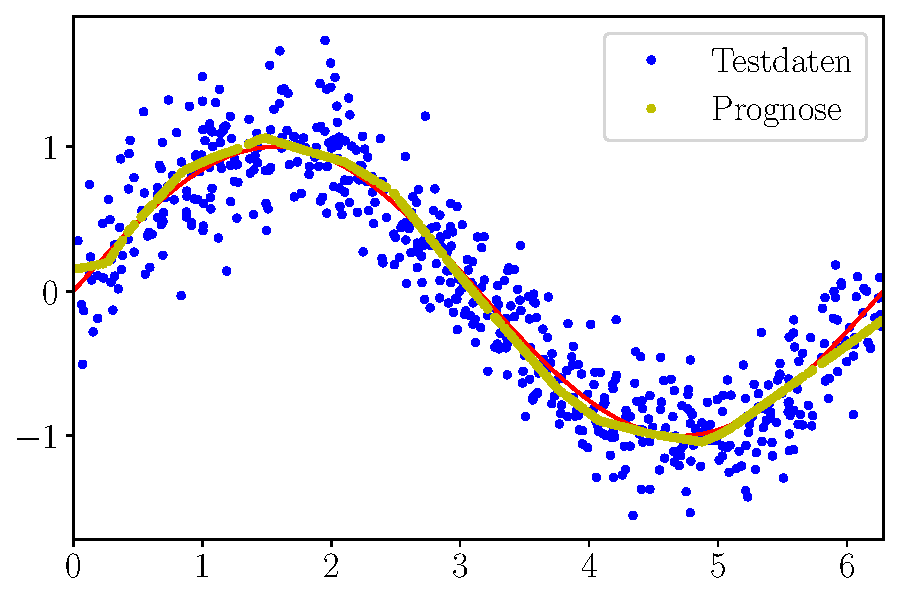
\includegraphics[width=\wMD]{first-nn/2-predictions.pdf}
  \caption{Ein Graph der Prognosen des verbesserten Modells gegenüber der Sollwerte aus dem
  \textit{test set} zusammen mit der Sinuskurve als Referenz}
  \label{fig:predictions-train-set}
\end{figure}

\section{Konvertieren des Modells nach TensorFlow Lite}
\label{sec:convert-model}
Nun, wo die gewünschte Qualität des Netztes erreicht
wurde, ist es Zeit, dieses umzuwandeln.
Das Modell soll für die Verwendung auf mobilen Geräten optimiert werden
und kompatibel mit der Edge TPU sein.
Hierfür wird Gebrauch von der TensorFlow Lite (TFLite) Bibliothek gemacht.
Wie in \autoref{sec:dl-mobile} untersucht,
besteht das Hauptziel der Konvertierung darin, die Modellgröße zu verringern
für schnellere Ausführung, kürzere Downloadzeiten und geringere RAM Nutzung.
Zuerst wird das normale Keras Modell gespeichert:
\begin{pythoncode}
model.save("sine_model.h5")
\end{pythoncode}
Keras verwendet das HDF5 Dateiformat
indem alle Informationen über das gespeicherte Netz enthalten sind,
inklusive der trainierten Gewichte, Bias-Werte und alle eingestellten
Parameter \parencite[314]{book:hands-on-ml}.
Anders als bei TensorFlow Lite werden durch Keras keine Optimierungsschritte
durchgeführt.
TFLite setzt eine speziell für Speicherplatz und Geschwindigkeit
optimierte Architektur ein,
die sich \textit{FlatBuffers} nennt.
\textit{FlatBuffers} sind eine von Google
entwickelte Technologie, ursprünglich entworfen für die Spieleentwicklung
und anderen leistungskritischen Anwendungen.
\textit{FlatBuffers} können ohne Vorverarbeitung direkt in den RAM
geladen werden, dies verringert die Ladezeit
und minimiert den Speicherfußabdruck \parencite[685]{book:hands-on-ml}.
Die Umwandlung geschieht durch die
\pythoninline{tf.lite.TFLiteConverter} Klasse:
\begin{pythoncode}
# Konvertierung von einem Keras Modell
converter = tf.lite.TFLiteConverter.from_keras_model(model)
tflite_model = converter.convert() # Gibt FlatBuffer Bytes zurück

def save_model(model, model_name):
    with open(model_name, "wb") as f:
        f.write(model)

# Schreibe die binären Daten in eine Datei
save_model(tflite_model, "sine_model.tflite")
\end{pythoncode}
Ein Vergleich der Modellgrößen zeigt schon jetzt einen riesigen Unterschied:
\begin{pyconcode}
>>> import os
>>> sine_original_size = os.path.getsize("sine_model.h5")
>>> print(f"Ursprüngliche Größe: {sine_original_size} bytes")
Ursprüngliche Größe: 25480 bytes
>>> sine_lite_size = os.path.getsize("sine_model.tflite")
>>> print(f"TFLite Größe: {sine_lite_size} bytes")
TFLite Größe: 4856 bytes
>>> print(f"Differenz: {sine_original_size - sine_lite_size} bytes")
Differenz: 20624 bytes
\end{pyconcode}
Das TFLite Modell ist um einiges kleiner als die ursprüngliche Datei,
kann aber noch nicht zusammen mit der Edge TPU verwendet werden.
\autoref{sec:train-evaluate-model} hat gezeigt,
dass die Gewichte einer Schicht als
\qty{32}{\bit} Gleitkommazahlen dargestellt werden.
Eine weitere Technik, um die Modellgröße zu verringern,
ist es, diese Bitbreite zu verkürzen.
Werden beispielsweise \qty{16}{\bit} Gleitkommazahlen verwendet,
kann die Dateigröße erneut Mal halbiert werden.
TensorFlow Lite kann allerdings noch weiter gehen, als dass, indem
alle Berechnungen als 8-Bit-Ganzzahloperationen dargestellt werden.
Dieser Prozess nennt sich Quantisierung
(engl. \textit{quantization}) und führt zu einer vierfachen Verkleinerung.
Für die Verwendung mit Edge TPUs ist dieser Schritt nicht optional,
da sie speziell dafür ausgerichtet sind,
mit ganzen Zahlen zu rechnen \parencite{online:models-on-edge-tpu}.
Quantisierung kann auf zwei Weisen durchgeführt werden:
Während dem Training (\textit{Quantization aware training})
und nach dem Training (\textit{Post-training quantization}).
Die Quantisierungsschritte sind für beide Verfahren ähnlich,
\textit{Post-training quantization} benötigt jedoch etwas weniger Vorbereitung,
weshalb es hier gezeigt wird.
Quantisierung untersucht alle Gewichte des Modells, um
den größten absoluten Wert $m$ zu finden. Der Bereich $[-m,m]$
wird anschließend auf die feste Länge $[-127,127]$
abgebildet \parencite[686]{book:hands-on-ml}.
Eine 8-bit-Ganzzahl wird durch die folgende Gleichung ap­pro­xi­mie­rt \parencite{DBLP:quantization}:
\begin{equation}
  r = S(q - Z)
  \label{eq:quant}
\end{equation}
Die Konstanten $S$ und $Z$ sind die Quantisierungsparameter.
$S$ ist die Skalierung (engl. \textit{scale}),
$Z$ ist der Nullpunkt (engl. \textit{zero point}),
$r$ ist die reale Gleitkommazahl und $q$ ist der quantisierte Wert
(in diesem Fall eine 8-bit-Ganzzahl).
Das Sinusmodell kann wie folgt quantisiert werden:
\begin{pythoncode}
# Konvertierung von einem Keras Modell
converter = tf.lite.TFLiteConverter.from_keras_model(model)
# Quantisiere alle festen Parameter (wie Gewichte und Bias-Werte)
converter.optimizations = [tf.lite.Optimize.DEFAULT]

# Ein repräsentativer Datensatz, damit neben den festen Parametern
# auch die Aktivierungen quantisiert werden können
# hierfür werden die Testdaten verwendet
def representative_dataset():
    for value in x_test:
        yield [value]

# Benutze den repräsentativen Datensatz
converter.representative_dataset = representative_dataset
# Werfe einen Fehler wenn eine Operation nicht quantisiert werden kann
converter.target_spec.supported_ops = [tf.lite.OpsSet.TFLITE_BUILTINS_INT8]
# Auch Ein- und Ausgaben sollen Ganzzahlen sein
converter.inference_input_type = tf.int8
converter.inference_output_type = tf.int8

# Konvertiere das Modell nach FlatBuffer
tflite_model = converter.convert()

# Speichere die binären Daten
save_model(tflite_model, "sine_model_quant.tflite")
\end{pythoncode}
Damit neben den Gewichten und Bias-Werten auch die Aktivierungen
quantisiert werden können, wird ein repräsentativer Datensatz benötigt.
Dieser Schritt ist nur relevant für \textit{Post-training quantization}.
Die Modellgröße des quantisierten Netzes kann
erneut verglichen werden:
\begin{pyconcode}
>>> sine_lite_size = os.path.getsize("sine_model.tflite")
>>> print(f"TFLite Größe: {sine_lite_size} bytes")
TFLite Größe: 4856 bytes
>>> sine_lite_quant_size = os.path.getsize("sine_model_quant.tflite")
>>> print(f"TFLite + Quantisierung Größe: {sine_lite_quant_size} bytes")
TFLite + Quantisierung Größe: 3280 bytes
>>> print(f"Differenz: {sine_lite_size - sine_lite_quant_size} bytes")
Differenz: 1576 bytes
\end{pyconcode}
Die Dateigröße wurde ein weiteres Mal reduziert, eine
vierfache Verkleinerung konnte jedoch nicht erreicht werden.
Dies hat den Grund, da das Netz von vornherein bereits
sehr klein ist und Gewichte und Bias-Werte neben anderen
Informationen wie dem Berechnugsgraphen nur einen kleinen
Teil der Gesamtgröße ausmachen \parencite[64]{book:tiny-ml}.
Für größere Modelle würde eine vierfache Verkleinerung
festgestellt werden. Das Netz ist nun vollständig
quantisiert und kann somit restlos auf der Edge TPU
ausgeführt werden. Davor muss das Modell aber noch kompiliert werden, dies
geht mithilfe des \consoleinline{edgetpu_compiler}:
\begin{consolecode}
$ edgetpu_compiler sine_model_quant.tflite
Edge TPU Compiler version 16.0.384591198
Started a compilation timeout timer of 180 seconds.

Model compiled successfully in 43 ms.

Input model: sine_model_quant.tflite
Output model: sine_model_quant_edgetpu.tflite
Operation log: sine_model_quant_edgetpu.log
[...]
Compilation succeeded!
\end{consolecode}
Das Projektverzeichnis enthält nun vier Modelldateien und eine Log-Datei:
\begin{consolecode}
$ ls | cat
[...]
sine_model.h5
sine_model.tflite
sine_model_quant.tflite
sine_model_quant_edgetpu.log
sine_model_quant_edgetpu.tflite
\end{consolecode}
Die Log-Datei birgt weitere nützliche Informationen:
\begin{consolecode}
$ cat sine_model_quant_edgetpu.log
Edge TPU Compiler version 16.0.384591198
Input: sine_model_quant.tflite
Output: sine_model_quant_edgetpu.tflite

Operator                       Count      Status

FULLY_CONNECTED                4          Mapped to Edge TPU
\end{consolecode}
Die Ausgabe bestätigt, dass alle vier Schichten des Netzes
(drei verborgene und eine Ausgabeschicht)
auf der Edge TPU ausgeführt werden.

\section{Ein Vergleich der Modelle}
Die soeben erstellten Modelle können nun verwendet werden, um
Vorhersagen zu machen.
Da die Fokussierung von TensorFlow Lite auf Geschwindigkeit
liegt, umfasst dieser Vorgang im Vergleich zu Keras einige
zusätzliche Schritte. Der folgende Programmausschnitt
wird das unquantisierte und für die Edpe TPU
kompilierte TFLite Modell verwenden, um über dem Testdatensatz Inferenzen
durchzuführen. Die Ergebnisse können dann mit den Prognosen
aus \autoref{fig:predictions-train-set} verglichen werden,
um festzustellen, ob durch die Quantisierung bemerkbare
Genauigkeitsverluste entstanden sind.
Anstatt wie in Keras einfach die \pythoninline{predict}
Methode aufzurufen, müssen in TFLite die folgenden
Schritte durchgeführt werden:
\begin{enumerate}
  \item Instanziiere ein \pythoninline{Interpreter} Objekt.
  \item Rufe eine Methode auf, um den
        \textit{FlatBuffer} in den Arbeitsspeicher zu laden.
  \item Schreibe die Netzeingaben in den Eingabetensor.
  \item Rufe das Modell auf.
  \item Lese die Netzausgaben aus dem Ausgabetensor.
\end{enumerate}
\begin{pythoncode}
import platform

# Plattformspezifische Bibliotheken für die Edge TPU
EDGETUP_LIB = {
    "Linux": "libedgetpu.so.1",
    "Darwin": "libedgetpu.1.dylib",
    "Windows": "edgetpu.dll",
}[platform.system()]

# 1. Instanziiere die Interpreter
# Dieses Modell wird auf der CPU ausgeführt
sine_model_cpu = tf.lite.Interpreter("sine_model.tflite")
# Dieses Modell wird auf der Edge TPU ausgeführt
sine_model_tpu = tf.lite.Interpreter(
    "sine_model_quant_edgetpu.tflite",
    experimental_delegates=[tf.lite.experimental.load_delegate(EDGETUP_LIB)]
)
\end{pythoncode}
Jedes Modell besitzt eine Liste von Eingabe- und Ausgabedetails
mit Informationen für jede Ein- und Ausgabeschicht des neuronalen Netzes.
Die folgenden Ausgaben sind gekürzt und zeigen nur die wichtigsten Werte:
\begin{pyconcode}
>>> # Das Edge-TPU-Modell mit ganzzahligen Ein- und Ausgaben und Quantisierung
>>> sine_model_tpu.get_input_details()
[{"index": 0,
  "shape": array([1, 1]),
  "dtype": numpy.int8,
  "quantization": (0.024590179324150085, -128)}]
>>> sine_model_tpu.get_output_details()
[{"index": 1,
  "shape": array([1, 1]),
  "dtype": numpy.int8,
  "quantization": (0.008226378820836544, -2)}]
>>> # Das CPU-Modell mit Gleitkommazahlen und keiner Quantisierung
>>> sine_model_cpu.get_input_details()
[{"index": 0,
  "shape": array([1, 1]),
  "dtype": numpy.float32,
  "quantization": (0.0, 0)}]
>>> sine_model_cpu.get_output_details()
[{"index": 12,
  "shape": array([1, 1]),
  "dtype": numpy.float32,
  "quantization": (0.0, 0)}]
>>> # Weitere nicht gezeigte Attribute (dieselben wie für alle anderen Details)
>>> sine_model_cpu.get_output_details()[0].keys()
dict_keys(["name", "index", "shape", "shape_signature", "dtype",
           "quantization", "quantization_parameters", "sparsity_parameters"])
\end{pyconcode}
Diese Informationen können nun verwendet werden, um die
restlichen Schritte durchzuführen:
\begin{pythoncode*}{escapeinside=||}
# 2. Weise den Arbeitsspeicher zu
sine_model_cpu.allocate_tensors()
sine_model_tpu.allocate_tensors()

input_details_cpu = sine_model_cpu.get_input_details()[0]
input_details_tpu = sine_model_tpu.get_input_details()[0]

output_details_cpu = sine_model_cpu.get_output_details()[0]
output_details_tpu = sine_model_tpu.get_output_details()[0]

# Vergleiche |\autoref{eq:quant}|
input_scale, input_zero_point = input_details_tpu["quantization"]
output_scale, output_zero_point = output_details_tpu["quantization"]

input_index_cpu = input_details_cpu["index"]
input_index_tpu = input_details_tpu["index"]

output_index_cpu = output_details_cpu["index"]
output_index_tpu = output_details_tpu["index"]

sine_model_cpu_predictions = []
sine_model_tpu_predictions = []

for value in x_test:
    float32_tensor = tf.expand_dims(value, axis=0)
    # Berechne den quantisierten Wert
    # |$q = (r / S) + Z$ \eqref{eq:quant}|
    int8_tensor = (value / input_scale) + input_zero_point
    int8_tensor = tf.cast(int8_tensor, dtype=tf.int8)
    int8_tensor = tf.expand_dims(int8_tensor, axis=0)
    
    # 3. Schreibe die Netzeingaben in den Eingabetensor
    sine_model_cpu.set_tensor(input_index_cpu, float32_tensor)
    sine_model_tpu.set_tensor(input_index_tpu, int8_tensor)

    # 4. Rufe das Modell auf
    sine_model_cpu.invoke()
    sine_model_tpu.invoke()
    
    # 5. Lese die Netzausgaben aus dem Ausgabetensor
    output = sine_model_cpu.get_tensor(output_index_cpu)[0,0]
    sine_model_cpu_predictions.append(output)
    output = sine_model_tpu.get_tensor(output_index_tpu)[0,0]
    # Berechne den realen Wert
    # |$r = S(q - Z)$ \eqref{eq:quant}|
    output = output_scale * (output - output_zero_point) 
    sine_model_tpu_predictions.append(output)
\end{pythoncode*}
Das in \autoref{fig:predictions-train-set} gezeigte Diagramm kann
durch die neuen Prognosen erweitert werden:
\begin{pythoncode}
plt.plot(x_test, y_test, "b.", label="Testdaten")
plt.plot(x_test, predictions_2, "ro", label="Keras Prognose")
plt.plot(x_test, sine_model_cpu_predictions, "yx", label="Lite CPU Prognose")
plt.plot(x_test, sine_model_tpu_predictions, "g+", label="Edge TPU Prognose")
plt.legend()
plt.show()
\end{pythoncode}
\begin{figure}[h!]
  \centering
  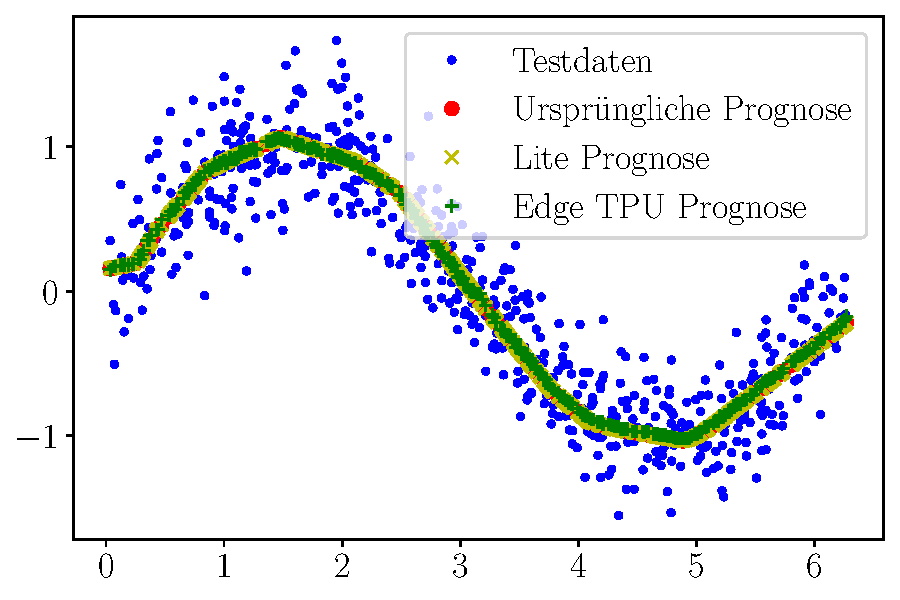
\includegraphics[width=\wMD]{first-nn/model-comparison.pdf}
  \caption{Ein Vergleich der Inferenzergebnisse des Keras-Modells, dem unquantisierten
  TFLite-CPU-Modell und dem quantisierten Edge-TPU-Modell}
  \label{fig:model-comparison}
\end{figure}
Es ist zu sehen, dass durch die Quantisierung keine oder nur kaum
zu bemerkende Genauigkeitsverluste entstanden sind.


\section{Ein Vergleich der Inferenzgeschwindigkeiten}
Es bleibt zu klären, ob durch die Ausführung des Modells
auf der Edge TPU eine Geschwindigkeitsverbesserung entsteht.
Hierfür werden im folgenden Python-Programm die
Inferenzgeschwindigkeiten verglichen.
Das Gerät benötigt eine angeschlossene Edge TPU
und das Python-Skript muss Zugriff auf
das \pythoninline{tflite_runtime} Paket haben.
Die Installation ist je nach Plattform eine unterschiedliche
(siehe hierfür die Coral AI und TensorFlow Dokumentation):
\begin{pythoncode}
import time
import tflite_runtime.interpreter as tflite
import platform
import numpy as np

# Die drei zu vergleichenden Modelle
sine_model_cpu = tflite.Interpreter("sine_model.tflite")
sine_model_quant_cpu = tflite.Interpreter("sine_model_quant.tflite")
sine_model_tpu = tflite.Interpreter("sine_model_quant_edgetpu.tflite",
    experimental_delegates=[tflite.load_delegate(EDGETUP_LIB)])

sine_model_cpu.allocate_tensors()
sine_model_quant_cpu.allocate_tensors()
sine_model_tpu.allocate_tensors()

rng = np.random.default_rng(42)

def measure_performance(model):
    input_details = model.get_input_details()[0]
    input_index = input_details["index"]
    input_shape = input_details["shape"]
    dtype = input_details["dtype"]

    # 1010 Testdaten im Bereich null bis sechs
    test_data = rng.random(size=[1010, *input_shape], dtype=np.float32) * 6

    if dtype == np.int8:
        # Skaliere die Eingaben für quantisierte Modelle
        input_scale, input_zero_point = input_details["quantization"]
        test_data = test_data / input_scale + input_zero_point
        test_data = test_data.astype(dtype)

    inference_times = []

    for i, value in enumerate(test_data):
        model.set_tensor(input_index, value)
        # Messe die Zeit der Ausführung in Millisekunden
        start = time.perf_counter()
        model.invoke()
        inference_time = (time.perf_counter() - start) * 1000
        # Überspringe die ersten Messungen damit vom Cache Gebrauch gemacht werden kann
        if i >= 10:
            inference_times.append(inference_time)

    return np.array(inference_times)

result = measure_performance(sine_model_cpu)
print(f"CPU benötigt {result.sum():.4f} ms - ({np.average(result):.4f})")
result = measure_performance(sine_model_quant_cpu)
print(f"CPU quantisiert benötigt {result.sum():.4f} ms - ({np.average(result):.4f})")
result = measure_performance(sine_model_tpu)
print(f"TPU benötigt {result.sum():.4f} ms - ({np.average(result):.4f})")
\end{pythoncode}
Die folgenden Befehle zeigen wie der obere Test durchgeführt wird.
In diesem Beispiel wurde der Benchmark
auf dem Siemens SIMATIC IOT2050 \eqref{fig:iot2050} ausgeführt:
\begin{consolecode}
$ mkdir benchmark && cd benchmark
$ python3 -m venv --system-site-packages venv
$ source venv/bin/activate
(venv) $ pip install --upgrade pip
(venv) $ pip install --ignore-installed numpy
(venv) $ wget "https://raw.githubusercontent.com/JensDll/bachelorarbeit-notebooks\
> /2.0.2/chapters/first-neural-network/benchmark/download.sh"
(venv) $ # Führe das Bash-Skript aus um die Modelle herunterzuladen
(venv) $ bash download.sh 2.0.2
(venv) $ cd models
(venv) $ python sine_benchmark.py
CPU benötigt 25.4106 ms - (0.0254)
CPU quantisiert benötigt 23.3715 ms - (0.0234)
TPU benötigt 209.9618 ms - (0.2100)
\end{consolecode}
\noindent
Das Modell, welches die Edge TPU verwendet, scheint um einiges
langsamer zu sein als diese, welche auf der CPU ausgeführt werden.
\autoref{fig:sine_model_inference_time} zeigt die Verteilung
der Messergebnisse eingetragenen in einem Diagramm.
\begin{figure}[h!]
  \centering
  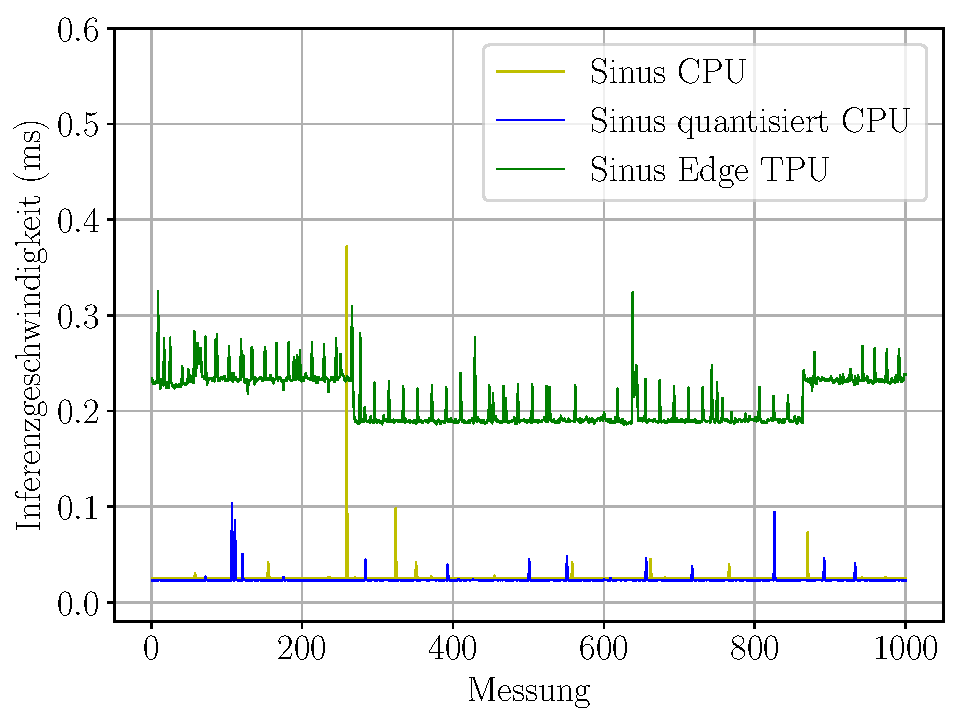
\includegraphics[width=\wMD]{first-nn/sine_model_inference_time.pdf}
  \caption{Ein Vergleich der Messergebnisse der Sinusmodelle
  auf dem Siemens SIMATIC IOT2050}
  \label{fig:sine_model_inference_time}
\end{figure}

\noindent
Die Edge TPU ist zweifellos langsamer, zusätzlich
sind die Zeiten des quantisierten Modells minimal besser.
Um zu bestätigen, dass die Edge TPU korrekt arbeitet,
wird ein zweiter Benchmark durchgeführt.
Dieses Mal aber mit einem Modell,
welches bereits getestet wurde.
Es wird das in \autoref{fig:ui-classification-example}
erwähnte Netz verwendet, um Insektenbilder zu unterscheiden:
\begin{pythoncode}
# Die zu vergleichenden Modelle
insect_model_cpu = tflite.Interpreter("mobilenet_v2_1.0_224_inat_insect_quant.tflite")
insect_model_tpu = tflite.Interpreter("mobilenet_v2_1.0_224_inat_insect_quant_edgetpu.tflite",
    experimental_delegates=[tflite.load_delegate(EDGETUP_LIB)])

insect_model_cpu.allocate_tensors()
insect_model_tpu.allocate_tensors()

rng = np.random.default_rng(42)

def measure_performance(model):
    input_details = model.get_input_details()[0]
    input_index = input_details["index"]
    input_shape = input_details["shape"][1:]

    # Ein zufälliges Testbild
    test_data = rng.integers(low=0, high=256, size=[1, *input_shape], dtype=np.uint8)

    inference_times = []

    for i in range(11):
        model.set_tensor(input_index, test_data)
        # Messe die Zeit der Ausführung in Millisekunden
        start = time.perf_counter()
        model.invoke()
        inference_time = (time.perf_counter() - start) * 1000
        # Überspringe die erste Messung
        if not i == 0:
            inference_times.append(inference_time)

    return np.array(inference_times)

result = measure_performance(insect_model_cpu)
print(f"CPU benötigt {result.sum():.4f} ms - ({np.average(result):.4f})")
result = measure_performance(insect_model_tpu)
print(f"TPU benötigt {result.sum():.4f} ms - ({np.average(result):.4f})")
\end{pythoncode}
Wurden die vorherigen Befehle ausgeführt,
kann auch dieses Programm einfach ausgeführt werden:
\begin{consolecode}
(venv) $ python mobilenet_benchmark.py
CPU benötigt 2027.1982 ms - (202.7198)
TPU benötigt 26.8095 ms - (2.6810)
\end{consolecode}
Die Edge TPU zeigt ein deutlich besseres Ergebnis.
Die Gründe für die langsamere Geschwindigkeit im ersten Test
sind unklar. Es gibt Diskussionen auf dem Google Coral Edge TPU
GitHub Repository (wie
\url{https://github.com/google-coral/edgetpu/issues/89}), in denen
ähnliche Ergebnisse gezeigt werden.
Die Edge TPU scheint für Netze mit vielen vollständig verbundenen Schichten
langsamer zu sein als die Ausführung desselben Netzes auf der CPU.
Wird die TPU hingegen für andere Netzarchitekturen
eingesetzt (wie dem \textit{Convolutional Neural Network} im zweiten Test),
führt dies zu einer wesentlich besseren Leistung.
Ein entwickeltes Modell sollte also immer zusammen
mit der verwendeten Hardware getestet werden, um die
Leistungsverbesserungen abzuschätzen und das mit der besten Geschwindigkeit auszuwählen.
Werden die oben durchgeführten Benchmarks vier weitere Male ausgeführt,
ergeben sich die Inferenzgeschwindigkeiten wie in \autoref{tab:benchmark-results}
zu sehen sind.
\begin{table}[h!]
  \centering
  \caption{Ein Vergleich der Inferenzgeschwindigkeiten, nachdem die
  gezeigten Benchmarks viermal hintereinander durchgeführt wurden}
  \label{tab:benchmark-results}
  \begin{tabular}{lSSSS}
    \toprule
                          & \multicolumn{4}{c}{Durchlauf (\unit{\milli\second})} \\ \cmidrule(){2-5}
    Modell                & 1         & 2         & 3         & 4                \\ \midrule
    Sinus CPU             & 24.7545   & 25.1723   & 24.7554   & 25.2206          \\
    Sinus quantisiert CPU & 22.9032   & 23.1907   & 22.7764   & 22.9355          \\
    Sinus Edge TPU        & 239.9419  & 211.3840  & 193.9379  & 228.0987         \\ \midrule
    MobileNet V2 CPU      & 2032.3503 & 2021.8814 & 2031.3118 & 2023.9531        \\
    MobileNet V2 Edge TPU & 27.5456   & 27.4322   & 27.5093   & 27.6126          \\ \bottomrule
  \end{tabular}
\end{table}
\begin{figure}[h!]
  \centering
  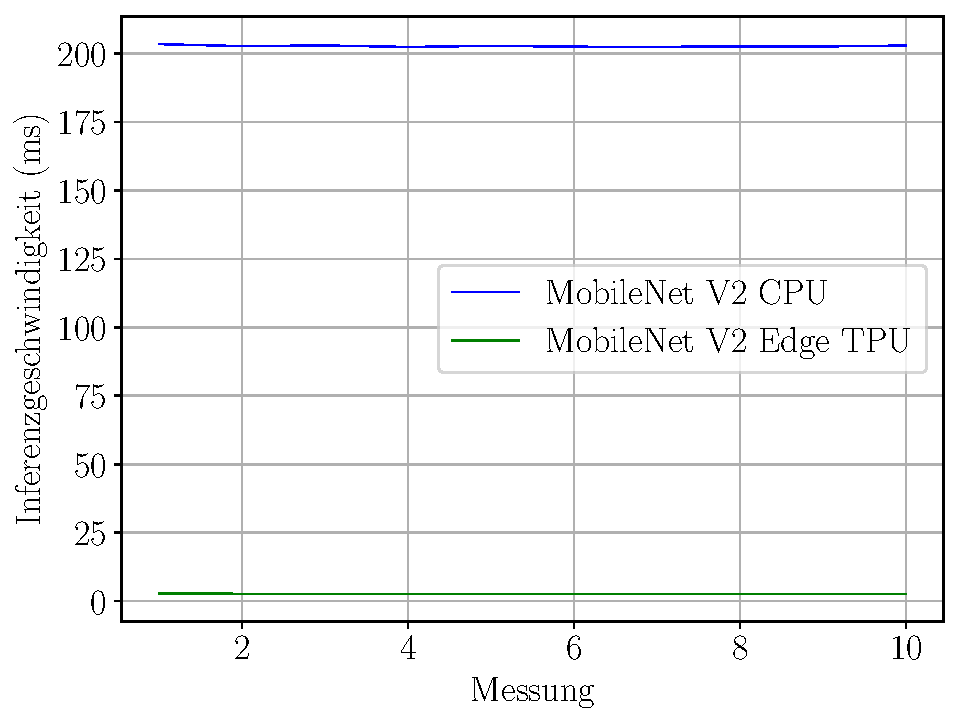
\includegraphics[width=\wMD]{first-nn/mobilenet_inference_time.pdf}
  \caption{Ein Vergleich der Messergebnisse des MobileNet V2
  Modells auf dem Siemens SIMATIC IOT2050}
  \label{fig:mobilenet_inference_time}
\end{figure}